\documentclass[aspectratio=169]{beamer}

% Minimal theme
\usetheme{default}
\usecolortheme{dove}

% Remove navigation symbols
\setbeamertemplate{navigation symbols}{}
\setbeamertemplate{footline}{%
  \hfill{\large\insertframenumber\,/\,\inserttotalframenumber}\hspace{0.8em}\vspace{0.5em}%
}

% Colors
\definecolor{popblue}{RGB}{52, 101, 164}
\definecolor{sampred}{RGB}{204, 0, 0}
\definecolor{paramgreen}{RGB}{0, 140, 70}
\definecolor{lightbg}{RGB}{245, 245, 250}
\definecolor{warnred}{RGB}{180, 40, 40}
\definecolor{orange1}{RGB}{220, 120, 0}
\definecolor{violet1}{RGB}{120, 50, 160}

\setbeamercolor{frametitle}{fg=popblue}
\setbeamercolor{title}{fg=popblue}

% Packages
\usepackage{pgfplots}
\usepackage{tikz}
\usetikzlibrary{shapes, arrows.meta, positioning, calc, decorations.pathreplacing, patterns}
\pgfplotsset{compat=1.18}
\usepackage{amsmath, amssymb}
\usepackage{array}
\usepackage{fontenc}

\title{From N-grams to LSTMs}
\subtitle{N-grams $\cdot$ Word2Vec $\cdot$ RNNs $\cdot$ LSTMs $\cdot$ Motivation for Attention}
\date{}

\begin{document}

% ============================================================
% TITLE
% ============================================================
\begin{frame}
\titlepage
\end{frame}

% ============================================================
% THE CORE PROBLEM
% ============================================================
\begin{frame}
\frametitle{The core problem}

\begin{center}
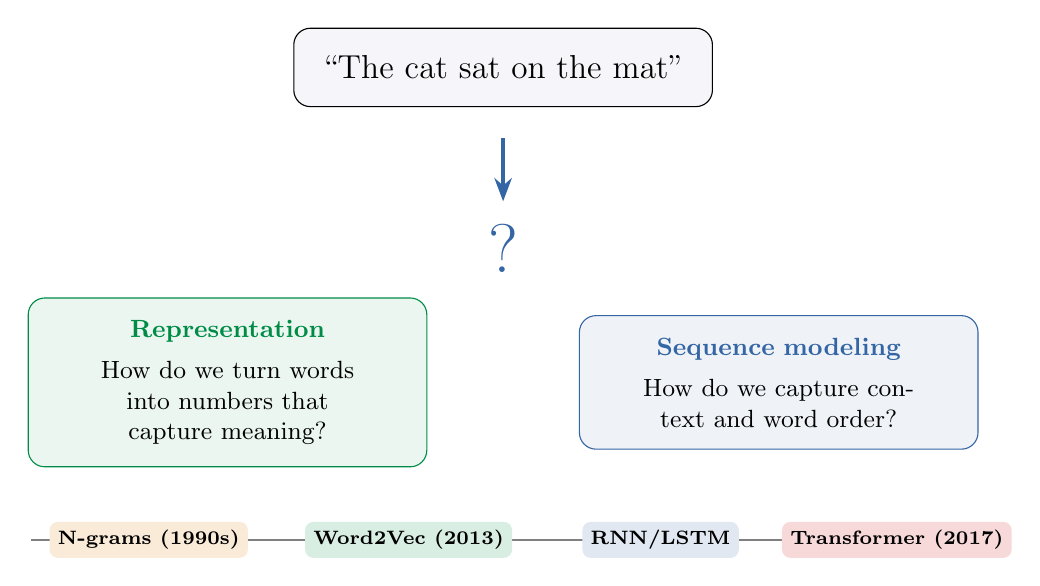
\begin{tikzpicture}
  % Sentence
  \node[draw, rounded corners=6pt, fill=lightbg, inner sep=10pt, font=\large] (sent) at (0, 2.5) {
    ``The cat sat on the mat''
  };

  % Arrow down
  \draw[-Stealth, very thick, popblue] (0, 1.6) -- (0, 0.8);
  \node[font=\Huge, text=popblue] at (0, 0.2) {?};

  % Two sub-problems
  \node[draw=paramgreen, fill=paramgreen!8, rounded corners=6pt, text width=4.5cm, align=center, inner sep=8pt, font=\small] at (-3.5, -1.5) {
    \textbf{\textcolor{paramgreen}{Representation}}\\[4pt]
    How do we turn words into numbers that capture meaning?
  };
  \node[draw=popblue, fill=popblue!8, rounded corners=6pt, text width=4.5cm, align=center, inner sep=8pt, font=\small] at (3.5, -1.5) {
    \textbf{\textcolor{popblue}{Sequence modeling}}\\[4pt]
    How do we capture context and word order?
  };

  % Timeline
  \draw[thick, -Stealth, gray] (-6, -3.5) -- (6, -3.5);
  \node[fill=orange1!15, rounded corners=3pt, inner sep=3pt, font=\scriptsize\bfseries] at (-4.5, -3.5) {N-grams (1990s)};
  \node[fill=paramgreen!15, rounded corners=3pt, inner sep=3pt, font=\scriptsize\bfseries] at (-1.2, -3.5) {Word2Vec (2013)};
  \node[fill=popblue!15, rounded corners=3pt, inner sep=3pt, font=\scriptsize\bfseries] at (2, -3.5) {RNN/LSTM};
  \node[fill=sampred!15, rounded corners=3pt, inner sep=3pt, font=\scriptsize\bfseries] at (5, -3.5) {Transformer (2017)};
\end{tikzpicture}
\end{center}
\end{frame}

% ============================================================
% N-GRAM LANGUAGE MODELS
% ============================================================
\begin{frame}
\frametitle{N-gram language models}

\vspace{-0.2cm}
\begin{center}
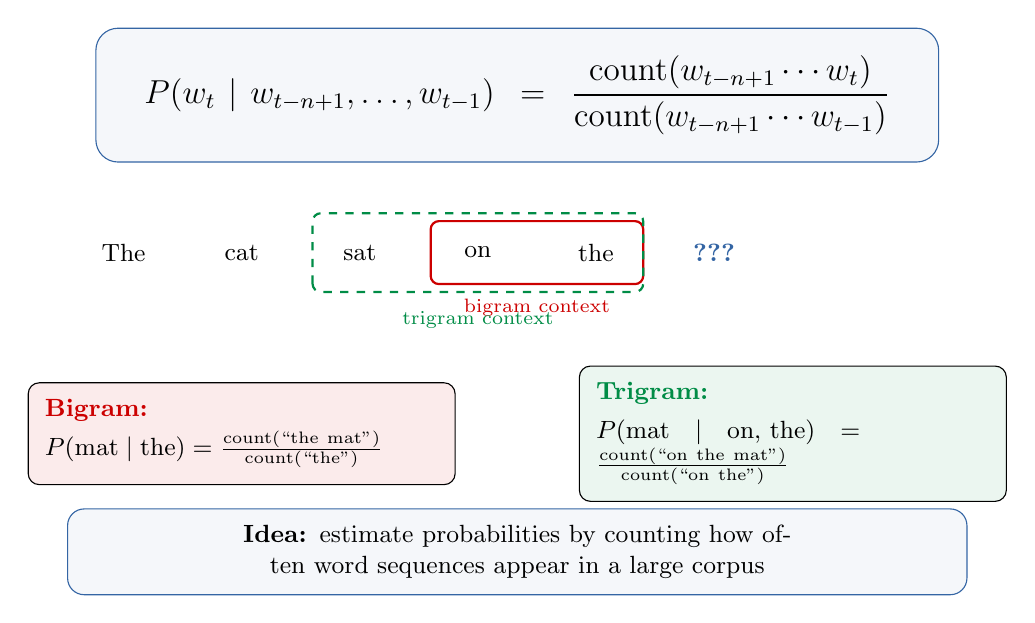
\begin{tikzpicture}
  % Formula
  \node[draw=popblue, fill=popblue!5, rounded corners=8pt, inner sep=10pt, text width=10cm, align=center] at (0, 3) {
    {\large $\displaystyle P(w_t \mid w_{t-n+1}, \ldots, w_{t-1}) \;=\; \frac{\text{count}(w_{t-n+1} \cdots w_t)}{\text{count}(w_{t-n+1} \cdots w_{t-1})}$}
  };

  % Sentence with sliding window
  \node[font=\small] (w1) at (-5, 1) {The};
  \node[font=\small] (w2) at (-3.5, 1) {cat};
  \node[font=\small] (w3) at (-2, 1) {sat};
  \node[font=\small] (w4) at (-0.5, 1) {on};
  \node[font=\small] (w5) at (1, 1) {the};
  \node[font=\small, text=popblue, font=\small\bfseries] (w6) at (2.5, 1) {???};

  % Bigram window
  \draw[thick, sampred, rounded corners=3pt] (-1.1, 0.6) rectangle (1.6, 1.4);
  \node[font=\scriptsize, text=sampred] at (0.25, 0.3) {bigram context};

  % Trigram window
  \draw[thick, paramgreen, rounded corners=3pt, dashed] (-2.6, 0.5) rectangle (1.6, 1.5);
  \node[font=\scriptsize, text=paramgreen] at (-0.5, 0.15) {trigram context};

  % Examples
  \node[draw, rounded corners=4pt, fill=sampred!8, text width=5cm, align=left, inner sep=6pt, font=\small] at (-3.5, -1.3) {
    \textbf{\textcolor{sampred}{Bigram:}}\\[3pt]
    $P(\text{mat} \mid \text{the}) = \frac{\text{count(``the mat'')}}{\text{count(``the'')}}$
  };
  \node[draw, rounded corners=4pt, fill=paramgreen!8, text width=5cm, align=left, inner sep=6pt, font=\small] at (3.5, -1.3) {
    \textbf{\textcolor{paramgreen}{Trigram:}}\\[3pt]
    $P(\text{mat} \mid \text{on, the}) = \frac{\text{count(``on the mat'')}}{\text{count(``on the'')}}$
  };

  % Key idea
  \node[draw=popblue, fill=popblue!5, rounded corners=6pt, text width=11cm, align=center, inner sep=6pt, font=\small] at (0, -2.8) {
    \textbf{Idea:} estimate probabilities by counting how often word sequences appear in a large corpus
  };
\end{tikzpicture}
\end{center}
\end{frame}

% ============================================================
% N-GRAM LIMITATIONS
% ============================================================
\begin{frame}
\frametitle{N-gram limitations}
\vspace{-0.3cm}
\begin{center}
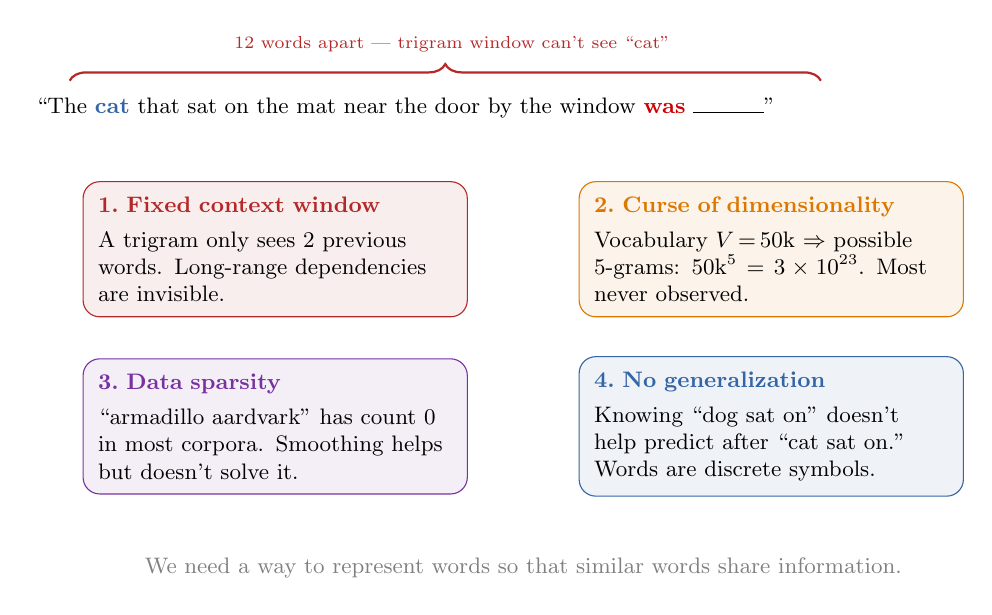
\begin{tikzpicture}[scale=0.9, transform shape]
  % Long sentence
  \node[font=\small, anchor=west] at (-7, 3.3) {``The \textbf{\textcolor{popblue}{cat}} that sat on the mat near the door by the window \textbf{\textcolor{sampred}{was}} \rule{1cm}{0.4pt}''};

  % Brace showing distance
  \draw[decorate, decoration={brace, amplitude=6pt, raise=2pt}, thick, warnred] (-6.4, 3.6) -- (4.2, 3.6);
  \node[font=\scriptsize, text=warnred] at (-1, 4.2) {12 words apart --- trigram window can't see ``cat''};

  % Four limitation boxes
  \node[draw=warnred, fill=warnred!8, rounded corners=6pt, text width=5cm, align=left, inner sep=6pt, font=\small] at (-3.5, 1.3) {
    \textbf{\textcolor{warnred}{1.~Fixed context window}}\\[3pt]
    A trigram only sees 2 previous words. Long-range dependencies are invisible.
  };
  \node[draw=orange1, fill=orange1!8, rounded corners=6pt, text width=5cm, align=left, inner sep=6pt, font=\small] at (3.5, 1.3) {
    \textbf{\textcolor{orange1}{2.~Curse of dimensionality}}\\[3pt]
    Vocabulary $V$\,=\,50k $\Rightarrow$ possible 5-grams: $50\text{k}^5 = 3\times10^{23}$. Most never observed.
  };
  \node[draw=violet1, fill=violet1!8, rounded corners=6pt, text width=5cm, align=left, inner sep=6pt, font=\small] at (-3.5, -1.2) {
    \textbf{\textcolor{violet1}{3.~Data sparsity}}\\[3pt]
    ``armadillo aardvark'' has count 0 in most corpora. Smoothing helps but doesn't solve it.
  };
  \node[draw=popblue, fill=popblue!8, rounded corners=6pt, text width=5cm, align=left, inner sep=6pt, font=\small] at (3.5, -1.2) {
    \textbf{\textcolor{popblue}{4.~No generalization}}\\[3pt]
    Knowing ``dog sat on'' doesn't help predict after ``cat sat on.'' Words are discrete symbols.
  };

  % Bottom
  \node[font=\small, text=gray, text width=11cm, align=center] at (0, -3.2) {
    We need a way to represent words so that similar words share information.
  };
\end{tikzpicture}
\end{center}
\end{frame}

% ============================================================
% ONE-HOT ENCODING
% ============================================================
\begin{frame}
\frametitle{One-hot encoding}

\begin{center}
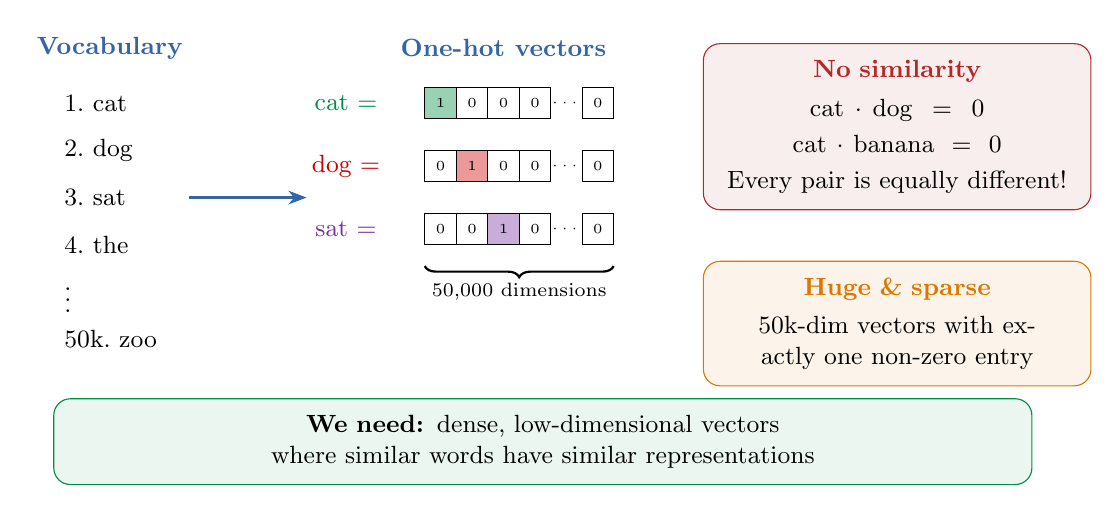
\begin{tikzpicture}
  % Vocabulary
  \node[font=\small\bfseries, text=popblue] at (-5.5, 3) {Vocabulary};
  \node[font=\small, anchor=west] at (-6.2, 2.3) {1.~cat};
  \node[font=\small, anchor=west] at (-6.2, 1.7) {2.~dog};
  \node[font=\small, anchor=west] at (-6.2, 1.1) {3.~sat};
  \node[font=\small, anchor=west] at (-6.2, 0.5) {4.~the};
  \node[font=\small, anchor=west] at (-6.2, -0.1) {$\vdots$};
  \node[font=\small, anchor=west] at (-6.2, -0.7) {50k.~zoo};

  % Arrow
  \draw[-Stealth, thick, popblue] (-4.5, 1.1) -- (-3, 1.1);

  % One-hot vectors
  \node[font=\small\bfseries, text=popblue] at (-0.5, 3) {One-hot vectors};

  % cat vector
  \node[font=\small, text=paramgreen] at (-2.5, 2.3) {cat =};
  \node[draw, minimum width=0.4cm, minimum height=0.4cm, fill=paramgreen!40, font=\tiny] at (-1.3, 2.3) {1};
  \node[draw, minimum width=0.4cm, minimum height=0.4cm, font=\tiny] at (-0.9, 2.3) {0};
  \node[draw, minimum width=0.4cm, minimum height=0.4cm, font=\tiny] at (-0.5, 2.3) {0};
  \node[draw, minimum width=0.4cm, minimum height=0.4cm, font=\tiny] at (-0.1, 2.3) {0};
  \node[font=\tiny] at (0.3, 2.3) {$\cdots$};
  \node[draw, minimum width=0.4cm, minimum height=0.4cm, font=\tiny] at (0.7, 2.3) {0};

  % dog vector
  \node[font=\small, text=sampred] at (-2.5, 1.5) {dog =};
  \node[draw, minimum width=0.4cm, minimum height=0.4cm, font=\tiny] at (-1.3, 1.5) {0};
  \node[draw, minimum width=0.4cm, minimum height=0.4cm, fill=sampred!40, font=\tiny] at (-0.9, 1.5) {1};
  \node[draw, minimum width=0.4cm, minimum height=0.4cm, font=\tiny] at (-0.5, 1.5) {0};
  \node[draw, minimum width=0.4cm, minimum height=0.4cm, font=\tiny] at (-0.1, 1.5) {0};
  \node[font=\tiny] at (0.3, 1.5) {$\cdots$};
  \node[draw, minimum width=0.4cm, minimum height=0.4cm, font=\tiny] at (0.7, 1.5) {0};

  % sat vector
  \node[font=\small, text=violet1] at (-2.5, 0.7) {sat =};
  \node[draw, minimum width=0.4cm, minimum height=0.4cm, font=\tiny] at (-1.3, 0.7) {0};
  \node[draw, minimum width=0.4cm, minimum height=0.4cm, font=\tiny] at (-0.9, 0.7) {0};
  \node[draw, minimum width=0.4cm, minimum height=0.4cm, fill=violet1!40, font=\tiny] at (-0.5, 0.7) {1};
  \node[draw, minimum width=0.4cm, minimum height=0.4cm, font=\tiny] at (-0.1, 0.7) {0};
  \node[font=\tiny] at (0.3, 0.7) {$\cdots$};
  \node[draw, minimum width=0.4cm, minimum height=0.4cm, font=\tiny] at (0.7, 0.7) {0};

  % Dimension annotation
  \draw[decorate, decoration={brace, amplitude=4pt, mirror, raise=2pt}, thick] (-1.5, 0.3) -- (0.9, 0.3);
  \node[font=\scriptsize] at (-0.3, -0.1) {50,000 dimensions};

  % Problems
  \node[draw=warnred, fill=warnred!8, rounded corners=6pt, text width=4.5cm, align=center, inner sep=6pt, font=\small] at (4.5, 2) {
    \textbf{\textcolor{warnred}{No similarity}}\\[3pt]
    $\text{cat} \cdot \text{dog} = 0$\\[2pt]
    $\text{cat} \cdot \text{banana} = 0$\\[2pt]
    Every pair is equally different!
  };

  \node[draw=orange1, fill=orange1!8, rounded corners=6pt, text width=4.5cm, align=center, inner sep=6pt, font=\small] at (4.5, -0.5) {
    \textbf{\textcolor{orange1}{Huge \& sparse}}\\[3pt]
    50k-dim vectors with exactly one non-zero entry
  };

  % Need
  \node[draw=paramgreen, fill=paramgreen!8, rounded corners=6pt, text width=12cm, align=center, inner sep=6pt, font=\small] at (0, -2) {
    \textbf{We need:} dense, low-dimensional vectors where similar words have similar representations
  };
\end{tikzpicture}
\end{center}
\end{frame}

% ============================================================
% WORD2VEC — DISTRIBUTIONAL HYPOTHESIS
% ============================================================
\begin{frame}
\frametitle{Word2Vec --- the distributional hypothesis}
\vspace{-0.3cm}
\begin{center}
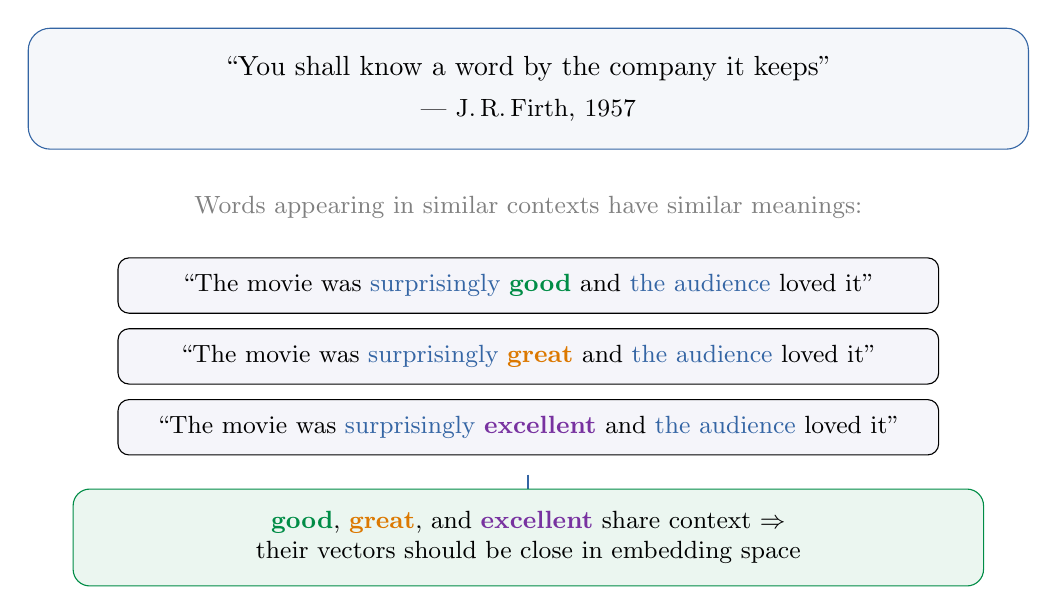
\begin{tikzpicture}
  % Quote
  \node[draw=popblue, fill=popblue!5, rounded corners=8pt, inner sep=10pt, text width=12cm, align=center, font=\normalsize] at (0, 3) {
    ``You shall know a word by the company it keeps''\\[3pt]
    {\small --- J.\,R.\,Firth, 1957}
  };

  % Two contexts for "good"
  \node[font=\small, text=gray] at (0, 1.5) {Words appearing in similar contexts have similar meanings:};

  % Context 1
  \node[draw, rounded corners=4pt, fill=lightbg, inner sep=6pt, font=\small, text width=10cm, align=center] at (0, 0.5) {
    ``The movie was \textcolor{popblue}{surprisingly} \textbf{\textcolor{paramgreen}{good}} and \textcolor{popblue}{the audience} loved it''
  };
  \node[draw, rounded corners=4pt, fill=lightbg, inner sep=6pt, font=\small, text width=10cm, align=center] at (0, -0.4) {
    ``The movie was \textcolor{popblue}{surprisingly} \textbf{\textcolor{orange1}{great}} and \textcolor{popblue}{the audience} loved it''
  };
  \node[draw, rounded corners=4pt, fill=lightbg, inner sep=6pt, font=\small, text width=10cm, align=center] at (0, -1.3) {
    ``The movie was \textcolor{popblue}{surprisingly} \textbf{\textcolor{violet1}{excellent}} and \textcolor{popblue}{the audience} loved it''
  };

  % Arrow to conclusion
  \draw[-Stealth, thick, popblue] (0, -1.9) -- (0, -2.4);

  % Conclusion
  \node[draw=paramgreen, fill=paramgreen!8, rounded corners=6pt, text width=11cm, align=center, inner sep=8pt, font=\small] at (0, -2.7) {
    \textbf{\textcolor{paramgreen}{good}}, \textbf{\textcolor{orange1}{great}}, and \textbf{\textcolor{violet1}{excellent}} share context $\Rightarrow$ their vectors should be close in embedding space
  };
\end{tikzpicture}
\end{center}
\end{frame}

% ============================================================
% WORD2VEC — CBOW & SKIP-GRAM
% ============================================================
\begin{frame}
\frametitle{Word2Vec --- CBOW \& Skip-gram}
\vspace{-0.3cm}
\begin{center}
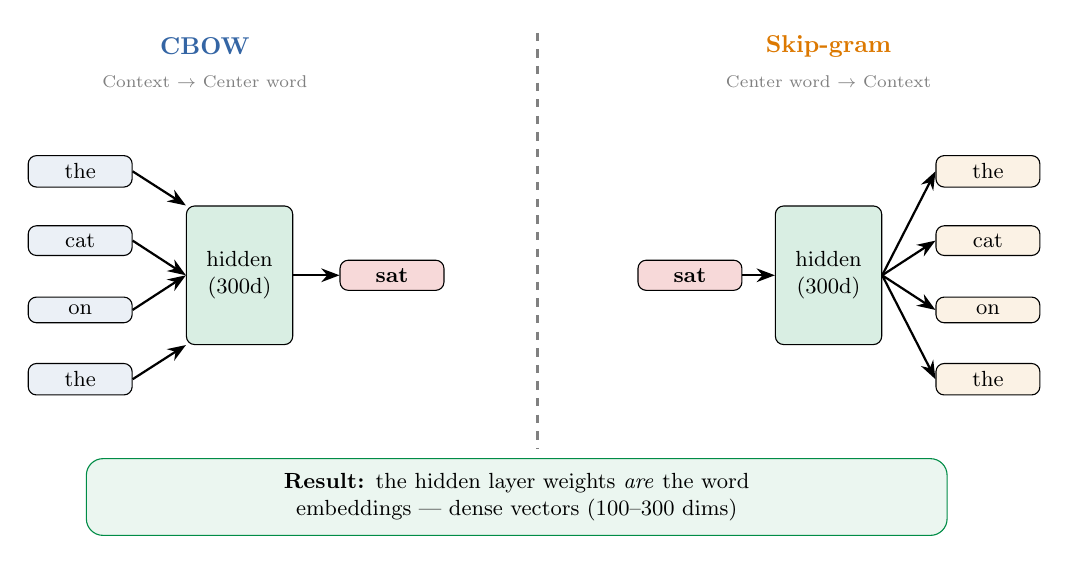
\begin{tikzpicture}[scale=0.88, transform shape]
  % ===== CBOW (left) =====
  \node[font=\normalsize\bfseries, text=popblue] at (-4.5, 3.3) {CBOW};
  \node[font=\scriptsize, text=gray] at (-4.5, 2.8) {Context $\rightarrow$ Center word};

  % Context inputs
  \node[draw, rounded corners=3pt, fill=popblue!10, minimum width=1.5cm, font=\small] (c1) at (-6.3, 1.5) {the};
  \node[draw, rounded corners=3pt, fill=popblue!10, minimum width=1.5cm, font=\small] (c2) at (-6.3, 0.5) {cat};
  \node[draw, rounded corners=3pt, fill=popblue!10, minimum width=1.5cm, font=\small] (c3) at (-6.3, -0.5) {on};
  \node[draw, rounded corners=3pt, fill=popblue!10, minimum width=1.5cm, font=\small] (c4) at (-6.3, -1.5) {the};

  % Hidden layer
  \node[draw, rounded corners=3pt, fill=paramgreen!15, minimum width=1.5cm, minimum height=2cm, font=\small, text width=1.3cm, align=center] (h1) at (-4.0, 0) {hidden\\(300d)};

  % Output
  \node[draw, rounded corners=3pt, fill=sampred!15, minimum width=1.5cm, font=\small\bfseries] (o1) at (-1.8, 0) {sat};

  % Arrows
  \draw[-Stealth, thick] (c1.east) -- (h1.north west);
  \draw[-Stealth, thick] (c2.east) -- (h1.west);
  \draw[-Stealth, thick] (c3.east) -- (h1.west);
  \draw[-Stealth, thick] (c4.east) -- (h1.south west);
  \draw[-Stealth, thick] (h1.east) -- (o1.west);

  % ===== Skip-gram (right) =====
  \node[font=\normalsize\bfseries, text=orange1] at (4.5, 3.3) {Skip-gram};
  \node[font=\scriptsize, text=gray] at (4.5, 2.8) {Center word $\rightarrow$ Context};

  % Input
  \node[draw, rounded corners=3pt, fill=sampred!15, minimum width=1.5cm, font=\small\bfseries] (i2) at (2.5, 0) {sat};

  % Hidden layer
  \node[draw, rounded corners=3pt, fill=paramgreen!15, minimum width=1.5cm, minimum height=2cm, font=\small, text width=1.3cm, align=center] (h2) at (4.5, 0) {hidden\\(300d)};

  % Context outputs
  \node[draw, rounded corners=3pt, fill=orange1!10, minimum width=1.5cm, font=\small] (o2a) at (6.8, 1.5) {the};
  \node[draw, rounded corners=3pt, fill=orange1!10, minimum width=1.5cm, font=\small] (o2b) at (6.8, 0.5) {cat};
  \node[draw, rounded corners=3pt, fill=orange1!10, minimum width=1.5cm, font=\small] (o2c) at (6.8, -0.5) {on};
  \node[draw, rounded corners=3pt, fill=orange1!10, minimum width=1.5cm, font=\small] (o2d) at (6.8, -1.5) {the};

  % Arrows
  \draw[-Stealth, thick] (i2.east) -- (h2.west);
  \draw[-Stealth, thick] (h2.east) -- (o2a.west);
  \draw[-Stealth, thick] (h2.east) -- (o2b.west);
  \draw[-Stealth, thick] (h2.east) -- (o2c.west);
  \draw[-Stealth, thick] (h2.east) -- (o2d.west);

  % Divider
  \draw[dashed, gray, thick] (0.3, 3.5) -- (0.3, -2.5);

  % Result
  \node[draw=paramgreen, fill=paramgreen!8, rounded corners=6pt, text width=12cm, align=center, inner sep=6pt, font=\small] at (0, -3.2) {
    \textbf{Result:} the hidden layer weights \emph{are} the word embeddings --- dense vectors (100--300 dims)
  };
\end{tikzpicture}
\end{center}
\end{frame}

% ============================================================
% WORD2VEC — EMERGENT PROPERTIES
% ============================================================
\begin{frame}
\frametitle{Word2Vec --- emergent properties}
\vspace{-0.3cm}
\begin{center}
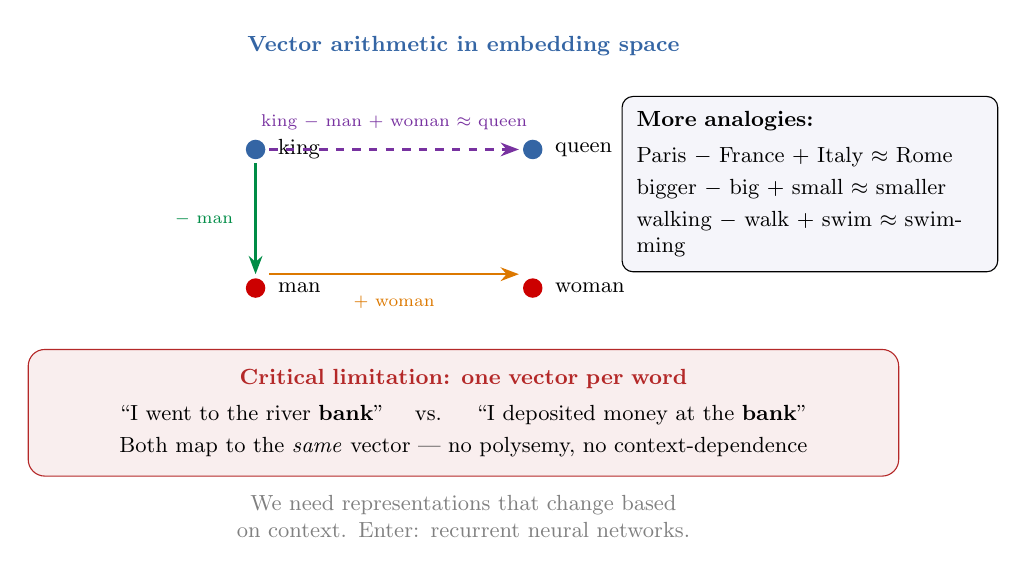
\begin{tikzpicture}[scale=0.88, transform shape]
  % 2D scatter of words
  \node[font=\small\bfseries, text=popblue] at (0, 3.5) {Vector arithmetic in embedding space};

  % King, Queen, Man, Woman
  \fill[popblue] (-3, 2) circle (4pt);
  \node[font=\small, anchor=west] at (-2.8, 2) {king};
  \fill[sampred] (-3, 0) circle (4pt);
  \node[font=\small, anchor=west] at (-2.8, 0) {man};
  \fill[popblue] (1, 2) circle (4pt);
  \node[font=\small, anchor=west] at (1.2, 2) {queen};
  \fill[sampred] (1, 0) circle (4pt);
  \node[font=\small, anchor=west] at (1.2, 0) {woman};

  % Arrows
  \draw[-Stealth, thick, paramgreen] (-3, 1.8) -- (-3, 0.2);
  \node[font=\scriptsize, text=paramgreen, anchor=east] at (-3.2, 1) {$-$ man};
  \draw[-Stealth, thick, orange1] (-2.8, 0.2) -- (0.8, 0.2);
  \node[font=\scriptsize, text=orange1] at (-1, -0.2) {$+$ woman};
  \draw[-Stealth, thick, violet1, dashed] (-2.8, 2) -- (0.8, 2);
  \node[font=\scriptsize, text=violet1] at (-1, 2.4) {king $-$ man $+$ woman $\approx$ queen};

  % More examples
  \node[draw, rounded corners=4pt, fill=lightbg, text width=5cm, align=left, inner sep=6pt, font=\small] at (5, 1.5) {
    \textbf{More analogies:}\\[4pt]
    Paris $-$ France $+$ Italy $\approx$ Rome\\[2pt]
    bigger $-$ big $+$ small $\approx$ smaller\\[2pt]
    walking $-$ walk $+$ swim $\approx$ swimming
  };

  % Limitation
  \node[draw=warnred, fill=warnred!8, rounded corners=6pt, text width=12cm, align=center, inner sep=8pt, font=\small] at (0, -1.8) {
    \textbf{\textcolor{warnred}{Critical limitation: one vector per word}}\\[4pt]
    ``I went to the river \textbf{bank}'' \quad vs. \quad ``I deposited money at the \textbf{bank}''\\[2pt]
    Both map to the \emph{same} vector --- no polysemy, no context-dependence
  };

  % What we need
  \node[font=\small, text=gray, text width=11cm, align=center] at (0, -3.3) {
    We need representations that change based on context. Enter: recurrent neural networks.
  };
\end{tikzpicture}
\end{center}
\end{frame}

% ============================================================
% RNNs
% ============================================================
\begin{frame}
\frametitle{Recurrent Neural Networks (RNNs)}

\begin{center}
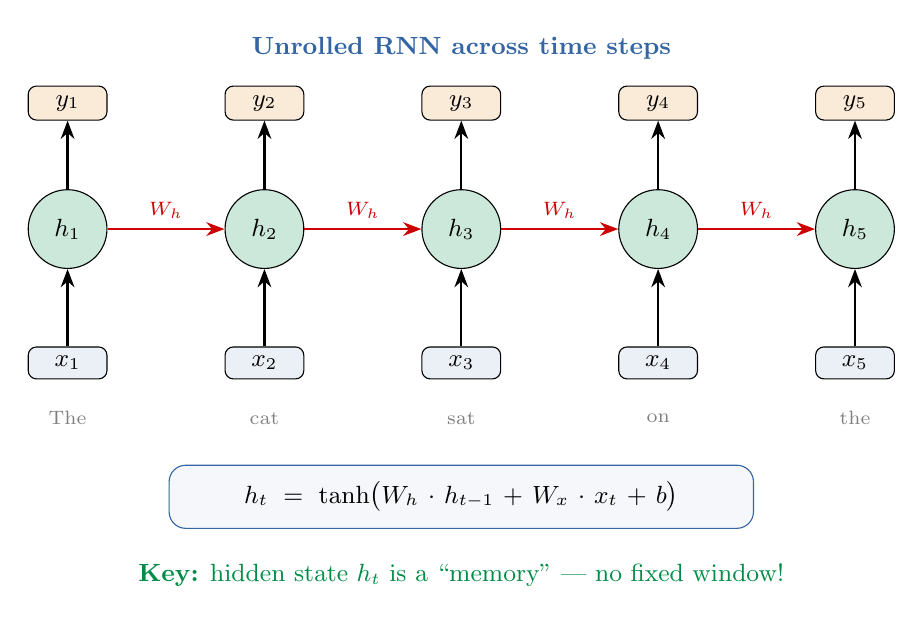
\begin{tikzpicture}
  % Unrolled RNN
  \node[font=\small\bfseries, text=popblue] at (0, 3.5) {Unrolled RNN across time steps};

  % Input tokens
  \node[draw, rounded corners=3pt, fill=popblue!10, minimum width=1cm, font=\small] (x1) at (-5, -0.5) {$x_1$};
  \node[draw, rounded corners=3pt, fill=popblue!10, minimum width=1cm, font=\small] (x2) at (-2.5, -0.5) {$x_2$};
  \node[draw, rounded corners=3pt, fill=popblue!10, minimum width=1cm, font=\small] (x3) at (0, -0.5) {$x_3$};
  \node[draw, rounded corners=3pt, fill=popblue!10, minimum width=1cm, font=\small] (x4) at (2.5, -0.5) {$x_4$};
  \node[draw, rounded corners=3pt, fill=popblue!10, minimum width=1cm, font=\small] (x5) at (5, -0.5) {$x_5$};

  % Hidden states
  \node[draw, circle, fill=paramgreen!20, minimum size=1cm, font=\small] (h1) at (-5, 1.2) {$h_1$};
  \node[draw, circle, fill=paramgreen!20, minimum size=1cm, font=\small] (h2) at (-2.5, 1.2) {$h_2$};
  \node[draw, circle, fill=paramgreen!20, minimum size=1cm, font=\small] (h3) at (0, 1.2) {$h_3$};
  \node[draw, circle, fill=paramgreen!20, minimum size=1cm, font=\small] (h4) at (2.5, 1.2) {$h_4$};
  \node[draw, circle, fill=paramgreen!20, minimum size=1cm, font=\small] (h5) at (5, 1.2) {$h_5$};

  % Outputs
  \node[draw, rounded corners=3pt, fill=orange1!15, minimum width=1cm, font=\small] (y1) at (-5, 2.8) {$y_1$};
  \node[draw, rounded corners=3pt, fill=orange1!15, minimum width=1cm, font=\small] (y2) at (-2.5, 2.8) {$y_2$};
  \node[draw, rounded corners=3pt, fill=orange1!15, minimum width=1cm, font=\small] (y3) at (0, 2.8) {$y_3$};
  \node[draw, rounded corners=3pt, fill=orange1!15, minimum width=1cm, font=\small] (y4) at (2.5, 2.8) {$y_4$};
  \node[draw, rounded corners=3pt, fill=orange1!15, minimum width=1cm, font=\small] (y5) at (5, 2.8) {$y_5$};

  % Vertical arrows
  \draw[-Stealth, thick] (x1) -- (h1);
  \draw[-Stealth, thick] (x2) -- (h2);
  \draw[-Stealth, thick] (x3) -- (h3);
  \draw[-Stealth, thick] (x4) -- (h4);
  \draw[-Stealth, thick] (x5) -- (h5);
  \draw[-Stealth, thick] (h1) -- (y1);
  \draw[-Stealth, thick] (h2) -- (y2);
  \draw[-Stealth, thick] (h3) -- (y3);
  \draw[-Stealth, thick] (h4) -- (y4);
  \draw[-Stealth, thick] (h5) -- (y5);

  % Recurrent arrows
  \draw[-Stealth, thick, sampred] (h1.east) -- (h2.west) node[midway, above, font=\scriptsize, text=sampred] {$W_h$};
  \draw[-Stealth, thick, sampred] (h2.east) -- (h3.west) node[midway, above, font=\scriptsize, text=sampred] {$W_h$};
  \draw[-Stealth, thick, sampred] (h3.east) -- (h4.west) node[midway, above, font=\scriptsize, text=sampred] {$W_h$};
  \draw[-Stealth, thick, sampred] (h4.east) -- (h5.west) node[midway, above, font=\scriptsize, text=sampred] {$W_h$};

  % Labels
  \node[font=\scriptsize, text=gray] at (-5, -1.2) {The};
  \node[font=\scriptsize, text=gray] at (-2.5, -1.2) {cat};
  \node[font=\scriptsize, text=gray] at (0, -1.2) {sat};
  \node[font=\scriptsize, text=gray] at (2.5, -1.2) {on};
  \node[font=\scriptsize, text=gray] at (5, -1.2) {the};

  % Formula
  \node[draw=popblue, fill=popblue!5, rounded corners=6pt, inner sep=6pt, font=\small, text width=7cm, align=center] at (0, -2.2) {
    $h_t = \tanh\!\big(W_h \cdot h_{t-1} + W_x \cdot x_t + b\big)$
  };

  % Key insight
  \node[font=\small, text=paramgreen] at (0, -3.2) {
    \textbf{Key:} hidden state $h_t$ is a ``memory'' --- no fixed window!
  };
\end{tikzpicture}
\end{center}
\end{frame}

% ============================================================
% VANISHING GRADIENT
% ============================================================
\begin{frame}
\frametitle{The vanishing gradient problem}
\vspace{-0.2cm}
\begin{center}
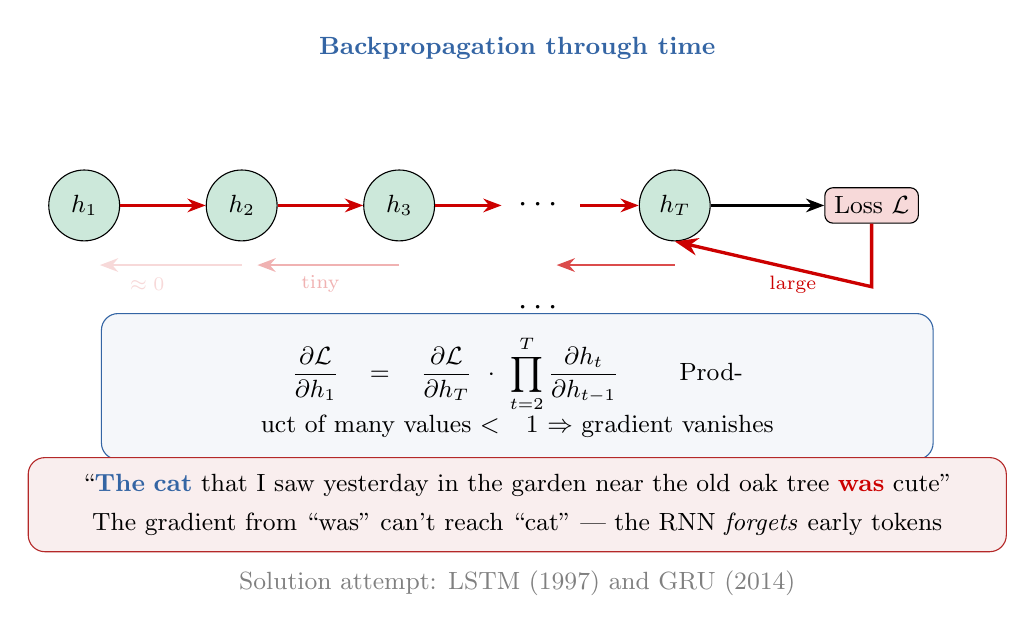
\begin{tikzpicture}
  % Unrolled RNN with fading gradients
  \node[font=\small\bfseries, text=popblue] at (0, 3.5) {Backpropagation through time};

  % Hidden states
  \node[draw, circle, fill=paramgreen!20, minimum size=0.9cm, font=\small] (h1) at (-5.5, 1.5) {$h_1$};
  \node[draw, circle, fill=paramgreen!20, minimum size=0.9cm, font=\small] (h2) at (-3.5, 1.5) {$h_2$};
  \node[draw, circle, fill=paramgreen!20, minimum size=0.9cm, font=\small] (h3) at (-1.5, 1.5) {$h_3$};
  \node[font=\large] at (0.3, 1.5) {$\cdots$};
  \node[draw, circle, fill=paramgreen!20, minimum size=0.9cm, font=\small] (h8) at (2, 1.5) {$h_T$};

  % Loss at end
  \node[draw, rounded corners=3pt, fill=sampred!15, font=\small] (loss) at (4.5, 1.5) {Loss $\mathcal{L}$};
  \draw[-Stealth, thick] (h8) -- (loss);

  % Forward arrows
  \draw[-Stealth, thick, sampred] (h1) -- (h2);
  \draw[-Stealth, thick, sampred] (h2) -- (h3);
  \draw[-Stealth, thick, sampred] (h3) -- (-0.2, 1.5);
  \draw[-Stealth, thick, sampred] (0.8, 1.5) -- (h8);

  % Gradient arrows going backward (fading)
  \draw[-Stealth, very thick, sampred] (loss.south) -- ++(0, -0.8) -- (h8.south);
  \draw[-Stealth, thick, sampred!70] (h8.south) ++(0, -0.3) -- ++(-1.5, 0);
  \node[font=\large] at (0.3, 0.2) {$\cdots$};
  \draw[-Stealth, thick, sampred!30] (h3.south) ++(0, -0.3) -- ++(-1.8, 0);
  \draw[-Stealth, thick, sampred!15] (h2.south) ++(0, -0.3) -- ++(-1.8, 0);

  % Gradient labels
  \node[font=\scriptsize, text=sampred] at (3.5, 0.5) {large};
  \node[font=\scriptsize, text=sampred!30] at (-2.5, 0.5) {tiny};
  \node[font=\scriptsize, text=sampred!15] at (-4.7, 0.5) {$\approx 0$};

  % Formula
  \node[draw=popblue, fill=popblue!5, rounded corners=6pt, inner sep=8pt, text width=10cm, align=center, font=\small] at (0, -0.8) {
    $\displaystyle \frac{\partial \mathcal{L}}{\partial h_1} = \frac{\partial \mathcal{L}}{\partial h_T} \cdot \prod_{t=2}^{T} \frac{\partial h_t}{\partial h_{t-1}}$ \qquad Product of many values $<1$ $\Rightarrow$ gradient vanishes
  };

  % Example
  \node[draw=warnred, fill=warnred!8, rounded corners=6pt, text width=12cm, align=center, inner sep=6pt, font=\small] at (0, -2.3) {
    ``\textbf{\textcolor{popblue}{The cat}} that I saw yesterday in the garden near the old oak tree \textbf{\textcolor{sampred}{was}} cute''\\[3pt]
    The gradient from ``was'' can't reach ``cat'' --- the RNN \emph{forgets} early tokens
  };

  \node[font=\small, text=gray] at (0, -3.3) {
    Solution attempt: LSTM (1997) and GRU (2014)
  };
\end{tikzpicture}
\end{center}
\end{frame}

% ============================================================
% LSTM
% ============================================================
\begin{frame}
\frametitle{LSTM --- Long Short-Term Memory}

\begin{center}
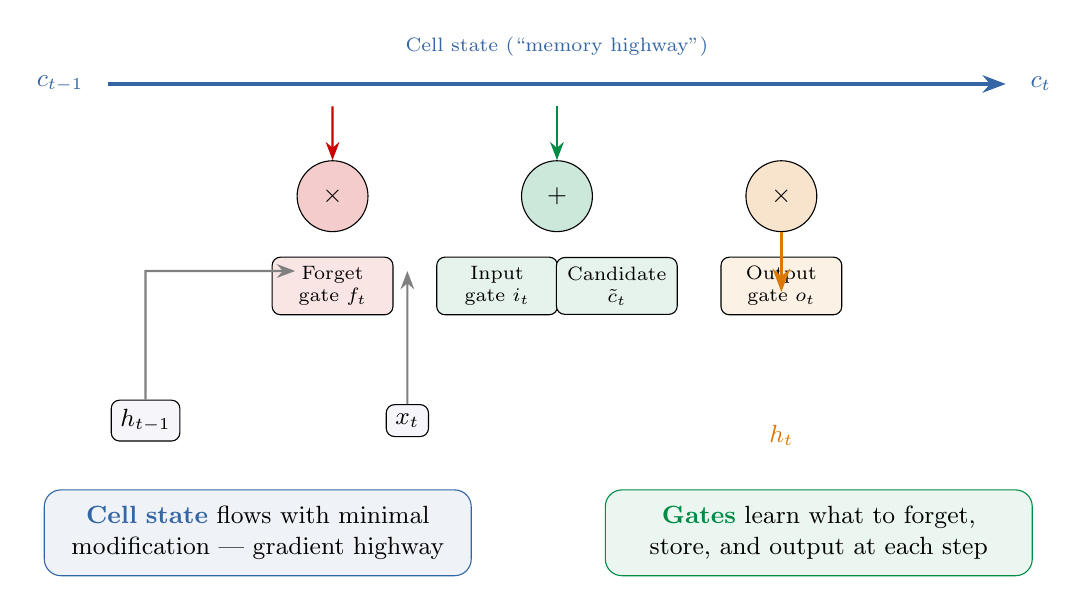
\begin{tikzpicture}[scale=0.95]
  % Cell state highway
  \draw[very thick, popblue, -Stealth] (-6, 3) -- (6, 3);
  \node[font=\small\bfseries, text=popblue, anchor=east] at (-6.2, 3) {$c_{t-1}$};
  \node[font=\small\bfseries, text=popblue, anchor=west] at (6.2, 3) {$c_t$};
  \node[font=\scriptsize, text=popblue] at (0, 3.5) {Cell state (``memory highway'')};

  % Forget gate
  \node[draw, circle, fill=sampred!20, minimum size=0.9cm, font=\small] (fg) at (-3, 1.5) {$\times$};
  \node[draw, rounded corners=3pt, fill=sampred!10, font=\scriptsize, text width=1.3cm, align=center] at (-3, 0.3) {Forget gate $f_t$};
  \draw[-Stealth, thick, sampred] (-3, 2.7) -- (fg);

  % Input gate
  \node[draw, circle, fill=paramgreen!20, minimum size=0.9cm, font=\small] (ig) at (0, 1.5) {$+$};
  \node[draw, rounded corners=3pt, fill=paramgreen!10, font=\scriptsize, text width=1.3cm, align=center] at (-0.8, 0.3) {Input gate $i_t$};
  \node[draw, rounded corners=3pt, fill=paramgreen!10, font=\scriptsize, text width=1.3cm, align=center] at (0.8, 0.3) {Candidate $\tilde{c}_t$};
  \draw[-Stealth, thick, paramgreen] (0, 2.7) -- (ig);

  % Output gate
  \node[draw, circle, fill=orange1!20, minimum size=0.9cm, font=\small] (og) at (3, 1.5) {$\times$};
  \node[draw, rounded corners=3pt, fill=orange1!10, font=\scriptsize, text width=1.3cm, align=center] at (3, 0.3) {Output gate $o_t$};

  % Hidden state output
  \draw[-Stealth, very thick, orange1] (og.south) -- ++(0, -0.8);
  \node[font=\small\bfseries, text=orange1] at (3, -1.7) {$h_t$};

  % h_{t-1} and x_t inputs
  \node[draw, rounded corners=3pt, fill=lightbg, font=\small] (ht1) at (-5.5, -1.5) {$h_{t-1}$};
  \node[draw, rounded corners=3pt, fill=lightbg, font=\small] (xt) at (-2, -1.5) {$x_t$};

  \draw[-Stealth, thick, gray] (ht1.north) -- (-5.5, 0.5) -- (-3.5, 0.5);
  \draw[-Stealth, thick, gray] (xt.north) -- (-2, 0.5);

  % Key insight boxes
  \node[draw=popblue, fill=popblue!8, rounded corners=6pt, text width=5cm, align=center, inner sep=6pt, font=\small] at (-4, -3) {
    \textbf{\textcolor{popblue}{Cell state}} flows with minimal modification --- gradient highway
  };
  \node[draw=paramgreen, fill=paramgreen!8, rounded corners=6pt, text width=5cm, align=center, inner sep=6pt, font=\small] at (3.5, -3) {
    \textbf{\textcolor{paramgreen}{Gates}} learn what to forget, store, and output at each step
  };
\end{tikzpicture}
\end{center}
\end{frame}

% ============================================================
% SEQUENCE-TO-SEQUENCE
% ============================================================
\begin{frame}
\frametitle{Sequence-to-sequence (Encoder--Decoder)}
\vspace{-0.4cm}
\begin{center}
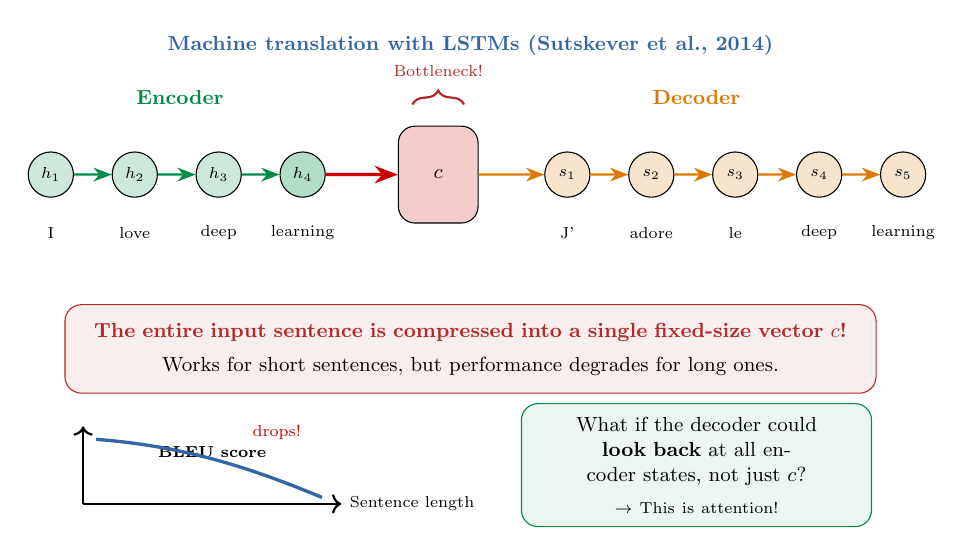
\begin{tikzpicture}[scale=0.82, transform shape]
  \node[font=\small\bfseries, text=popblue] at (0, 3.5) {Machine translation with LSTMs (Sutskever et al., 2014)};

  % ===== Encoder =====
  \node[font=\small\bfseries, text=paramgreen] at (-4.5, 2.7) {Encoder};

  % Encoder hidden states
  \node[draw, circle, fill=paramgreen!20, minimum size=0.7cm, font=\scriptsize] (e1) at (-6.5, 1.5) {$h_1$};
  \node[draw, circle, fill=paramgreen!20, minimum size=0.7cm, font=\scriptsize] (e2) at (-5.2, 1.5) {$h_2$};
  \node[draw, circle, fill=paramgreen!20, minimum size=0.7cm, font=\scriptsize] (e3) at (-3.9, 1.5) {$h_3$};
  \node[draw, circle, fill=paramgreen!30, minimum size=0.7cm, font=\scriptsize] (e4) at (-2.6, 1.5) {$h_4$};

  \draw[-Stealth, thick, paramgreen] (e1) -- (e2);
  \draw[-Stealth, thick, paramgreen] (e2) -- (e3);
  \draw[-Stealth, thick, paramgreen] (e3) -- (e4);

  % Encoder inputs
  \node[font=\scriptsize] at (-6.5, 0.6) {I};
  \node[font=\scriptsize] at (-5.2, 0.6) {love};
  \node[font=\scriptsize] at (-3.9, 0.6) {deep};
  \node[font=\scriptsize] at (-2.6, 0.6) {learning};

  % Context vector (bottleneck!)
  \node[draw, rounded corners=6pt, fill=sampred!20, minimum width=1cm, minimum height=1.5cm, font=\small, text width=1cm, align=center] (ctx) at (-0.5, 1.5) {\textbf{$c$}};
  \draw[-Stealth, very thick, sampred] (e4) -- (ctx);

  % Bottleneck annotation
  \draw[decorate, decoration={brace, amplitude=5pt, raise=2pt}, thick, warnred] (-0.9, 2.5) -- (-0.1, 2.5);
  \node[font=\scriptsize, text=warnred] at (-0.5, 3.1) {Bottleneck!};

  % ===== Decoder =====
  \node[font=\small\bfseries, text=orange1] at (3.5, 2.7) {Decoder};

  \node[draw, circle, fill=orange1!20, minimum size=0.7cm, font=\scriptsize] (d1) at (1.5, 1.5) {$s_1$};
  \node[draw, circle, fill=orange1!20, minimum size=0.7cm, font=\scriptsize] (d2) at (2.8, 1.5) {$s_2$};
  \node[draw, circle, fill=orange1!20, minimum size=0.7cm, font=\scriptsize] (d3) at (4.1, 1.5) {$s_3$};
  \node[draw, circle, fill=orange1!20, minimum size=0.7cm, font=\scriptsize] (d4) at (5.4, 1.5) {$s_4$};
  \node[draw, circle, fill=orange1!20, minimum size=0.7cm, font=\scriptsize] (d5) at (6.7, 1.5) {$s_5$};

  \draw[-Stealth, thick, orange1] (ctx) -- (d1);
  \draw[-Stealth, thick, orange1] (d1) -- (d2);
  \draw[-Stealth, thick, orange1] (d2) -- (d3);
  \draw[-Stealth, thick, orange1] (d3) -- (d4);
  \draw[-Stealth, thick, orange1] (d4) -- (d5);

  % Decoder outputs
  \node[font=\scriptsize] at (1.5, 0.6) {J'};
  \node[font=\scriptsize] at (2.8, 0.6) {adore};
  \node[font=\scriptsize] at (4.1, 0.6) {le};
  \node[font=\scriptsize] at (5.4, 0.6) {deep};
  \node[font=\scriptsize] at (6.7, 0.6) {learning};

  % Problem box
  \node[draw=warnred, fill=warnred!8, rounded corners=6pt, text width=12cm, align=center, inner sep=8pt, font=\small] at (0, -1.2) {
    \textbf{\textcolor{warnred}{The entire input sentence is compressed into a single fixed-size vector $c$!}}\\[4pt]
    Works for short sentences, but performance degrades for long ones.
  };

  % BLEU vs length sketch
  \node[font=\scriptsize\bfseries] at (-4, -2.8) {BLEU score};
  \draw[thick, ->] (-6, -3.6) -- (-2, -3.6) node[right, font=\scriptsize] {Sentence length};
  \draw[thick, ->] (-6, -3.6) -- (-6, -2.4);
  \draw[very thick, popblue] (-5.8, -2.6) .. controls (-4.5, -2.7) and (-3.5, -3.0) .. (-2.3, -3.5);
  \node[font=\scriptsize, text=sampred] at (-3, -2.5) {drops!};

  % Teaser
  \node[draw=paramgreen, fill=paramgreen!8, rounded corners=6pt, text width=5cm, align=center, inner sep=6pt, font=\small] at (3.5, -3) {
    What if the decoder could \textbf{look back} at all encoder states, not just $c$?\\[3pt]
    {\scriptsize $\rightarrow$ This is attention!}
  };
\end{tikzpicture}
\end{center}
\end{frame}

% ============================================================
% WHY LSTMS ARE NOT ENOUGH — BOTTLENECK
% ============================================================
\begin{frame}
\frametitle{Why LSTMs are not enough --- the bottleneck}
\vspace{-0.3cm}
\begin{center}
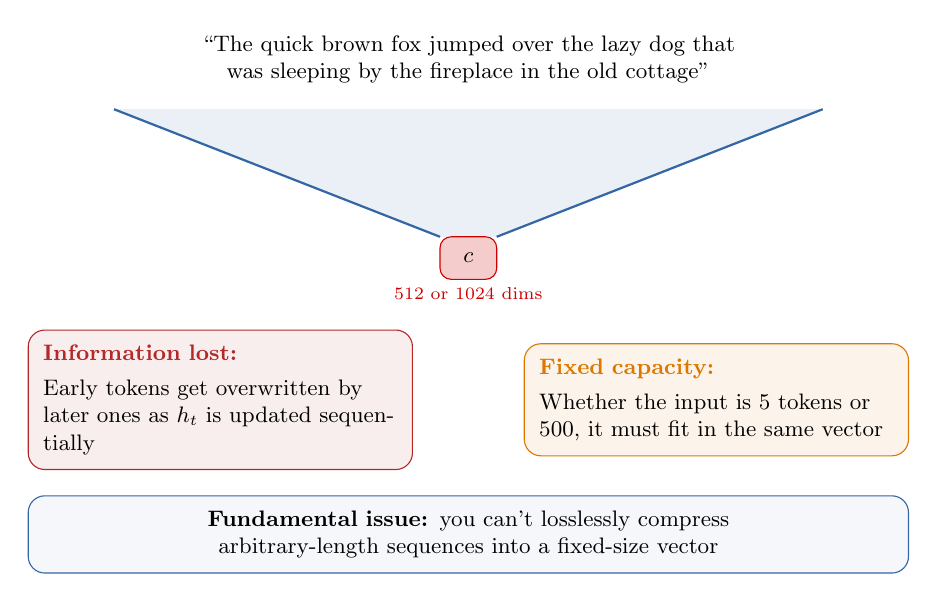
\begin{tikzpicture}[scale=0.9, transform shape]
  % Funnel visualization
  % Wide input
  \node[font=\small, text width=10cm, align=center] at (0, 3.5) {
    ``The quick brown fox jumped over the lazy dog that was sleeping by the fireplace in the old cottage''
  };

  % Funnel shape
  \fill[popblue!10] (-5, 2.8) -- (-0.4, 1) -- (0.4, 1) -- (5, 2.8) -- cycle;
  \draw[thick, popblue] (-5, 2.8) -- (-0.4, 1);
  \draw[thick, popblue] (5, 2.8) -- (0.4, 1);

  % Bottleneck vector
  \node[draw=sampred, fill=sampred!20, rounded corners=4pt, minimum width=0.8cm, minimum height=0.6cm, font=\small\bfseries] at (0, 0.7) {$c$};
  \node[font=\scriptsize, text=sampred] at (0, 0.2) {512 or 1024 dims};

  % What gets lost
  \node[draw=warnred, fill=warnred!8, rounded corners=6pt, text width=5cm, align=left, inner sep=6pt, font=\small] at (-3.5, -1.3) {
    \textbf{\textcolor{warnred}{Information lost:}}\\[3pt]
    Early tokens get overwritten by later ones as $h_t$ is updated sequentially
  };
  \node[draw=orange1, fill=orange1!8, rounded corners=6pt, text width=5cm, align=left, inner sep=6pt, font=\small] at (3.5, -1.3) {
    \textbf{\textcolor{orange1}{Fixed capacity:}}\\[3pt]
    Whether the input is 5 tokens or 500, it must fit in the same vector
  };

  % Key point
  \node[draw=popblue, fill=popblue!5, rounded corners=6pt, text width=12cm, align=center, inner sep=6pt, font=\small] at (0, -3.2) {
    \textbf{Fundamental issue:} you can't losslessly compress arbitrary-length sequences into a fixed-size vector
  };
\end{tikzpicture}
\end{center}
\end{frame}

% ============================================================
% WHY LSTMS ARE NOT ENOUGH — SEQUENTIAL
% ============================================================
\begin{frame}
\frametitle{Why LSTMs are not enough --- sequential processing}
\vspace{-0.2cm}
\begin{center}
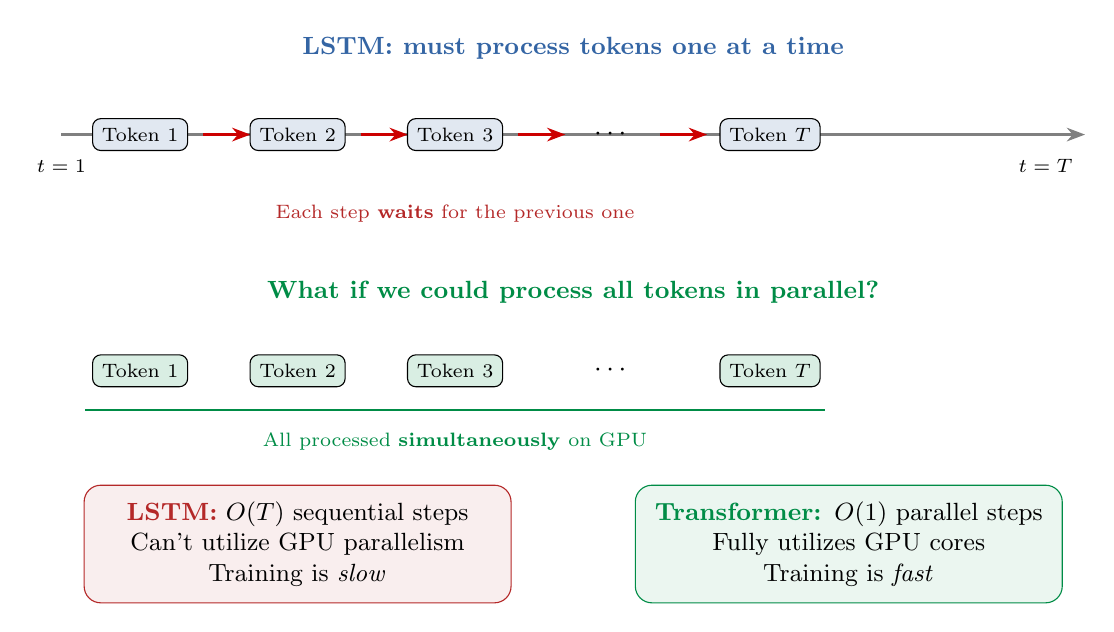
\begin{tikzpicture}
  % Sequential timeline
  \node[font=\small\bfseries, text=popblue] at (0, 3.3) {LSTM: must process tokens one at a time};

  % Timeline
  \draw[thick, -Stealth, gray] (-6.5, 2.2) -- (6.5, 2.2);
  \node[font=\scriptsize] at (-6.5, 1.8) {$t=1$};
  \node[font=\scriptsize] at (6, 1.8) {$t=T$};

  % Sequential boxes
  \node[draw, rounded corners=3pt, fill=popblue!15, minimum width=1.2cm, font=\scriptsize] at (-5.5, 2.2) {Token 1};
  \draw[-Stealth, thick, sampred] (-4.7, 2.2) -- (-4.1, 2.2);
  \node[draw, rounded corners=3pt, fill=popblue!15, minimum width=1.2cm, font=\scriptsize] at (-3.5, 2.2) {Token 2};
  \draw[-Stealth, thick, sampred] (-2.7, 2.2) -- (-2.1, 2.2);
  \node[draw, rounded corners=3pt, fill=popblue!15, minimum width=1.2cm, font=\scriptsize] at (-1.5, 2.2) {Token 3};
  \draw[-Stealth, thick, sampred] (-0.7, 2.2) -- (-0.1, 2.2);
  \node[font=\normalsize] at (0.5, 2.2) {$\cdots$};
  \draw[-Stealth, thick, sampred] (1.1, 2.2) -- (1.7, 2.2);
  \node[draw, rounded corners=3pt, fill=popblue!15, minimum width=1.2cm, font=\scriptsize] at (2.5, 2.2) {Token $T$};

  % Wait annotation
  \node[font=\scriptsize, text=warnred] at (-1.5, 1.2) {Each step \textbf{waits} for the previous one};

  % Parallel alternative
  \node[font=\small\bfseries, text=paramgreen] at (0, 0.2) {What if we could process all tokens in parallel?};

  % Parallel boxes
  \node[draw, rounded corners=3pt, fill=paramgreen!15, minimum width=1.2cm, font=\scriptsize] at (-5.5, -0.8) {Token 1};
  \node[draw, rounded corners=3pt, fill=paramgreen!15, minimum width=1.2cm, font=\scriptsize] at (-3.5, -0.8) {Token 2};
  \node[draw, rounded corners=3pt, fill=paramgreen!15, minimum width=1.2cm, font=\scriptsize] at (-1.5, -0.8) {Token 3};
  \node[font=\normalsize] at (0.5, -0.8) {$\cdots$};
  \node[draw, rounded corners=3pt, fill=paramgreen!15, minimum width=1.2cm, font=\scriptsize] at (2.5, -0.8) {Token $T$};

  % All at once annotation
  \draw[thick, paramgreen] (-6.2, -1.3) -- (3.2, -1.3);
  \node[font=\scriptsize, text=paramgreen] at (-1.5, -1.7) {All processed \textbf{simultaneously} on GPU};

  % Comparison
  \node[draw=warnred, fill=warnred!8, rounded corners=6pt, text width=5cm, align=center, inner sep=6pt, font=\small] at (-3.5, -3) {
    \textbf{\textcolor{warnred}{LSTM:}} $O(T)$ sequential steps\\
    Can't utilize GPU parallelism\\
    Training is \emph{slow}
  };
  \node[draw=paramgreen, fill=paramgreen!8, rounded corners=6pt, text width=5cm, align=center, inner sep=6pt, font=\small] at (3.5, -3) {
    \textbf{\textcolor{paramgreen}{Transformer:}} $O(1)$ parallel steps\\
    Fully utilizes GPU cores\\
    Training is \emph{fast}
  };
\end{tikzpicture}
\end{center}
\end{frame}

% ============================================================
% WHY LSTMS ARE NOT ENOUGH — LONG-RANGE
% ============================================================
\begin{frame}
\frametitle{Why LSTMs are not enough --- long-range dependencies}
\vspace{-0.3cm}
\begin{center}
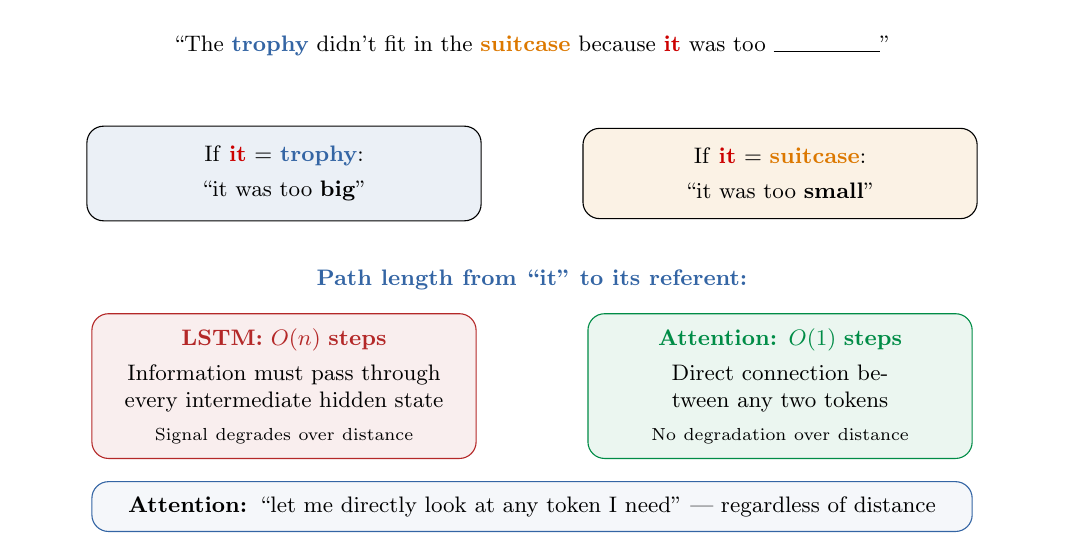
\begin{tikzpicture}[scale=0.9, transform shape]
  % Example sentence
  \node[font=\small, text width=14cm, align=center] at (0, 3) {
    ``The \textbf{\textcolor{popblue}{trophy}} didn't fit in the \textbf{\textcolor{orange1}{suitcase}} because \textbf{\textcolor{sampred}{it}} was too \rule{1.5cm}{0.4pt}''
  };

  % Two interpretations
  \node[draw, rounded corners=6pt, fill=popblue!10, text width=5cm, align=center, inner sep=8pt, font=\small] at (-3.5, 1.2) {
    If \textbf{\textcolor{sampred}{it}} = \textbf{\textcolor{popblue}{trophy}}:\\[3pt]
    ``it was too \textbf{big}''
  };
  \node[draw, rounded corners=6pt, fill=orange1!10, text width=5cm, align=center, inner sep=8pt, font=\small] at (3.5, 1.2) {
    If \textbf{\textcolor{sampred}{it}} = \textbf{\textcolor{orange1}{suitcase}}:\\[3pt]
    ``it was too \textbf{small}''
  };

  % Path length comparison
  \node[font=\small\bfseries, text=popblue] at (0, -0.3) {Path length from ``it'' to its referent:};

  % LSTM path
  \node[draw=warnred, fill=warnred!8, rounded corners=6pt, text width=5cm, align=center, inner sep=6pt, font=\small] at (-3.5, -1.8) {
    \textbf{\textcolor{warnred}{LSTM: $O(n)$ steps}}\\[3pt]
    Information must pass through every intermediate hidden state\\[2pt]
    {\scriptsize Signal degrades over distance}
  };

  % Transformer path
  \node[draw=paramgreen, fill=paramgreen!8, rounded corners=6pt, text width=5cm, align=center, inner sep=6pt, font=\small] at (3.5, -1.8) {
    \textbf{\textcolor{paramgreen}{Attention: $O(1)$ steps}}\\[3pt]
    Direct connection between any two tokens\\[2pt]
    {\scriptsize No degradation over distance}
  };

  % Bottom teaser
  \node[draw=popblue, fill=popblue!5, rounded corners=6pt, text width=12cm, align=center, inner sep=6pt, font=\small] at (0, -3.5) {
    \textbf{Attention:} ``let me directly look at any token I need'' --- regardless of distance
  };
\end{tikzpicture}
\end{center}
\end{frame}

% ============================================================
% THE STAGE IS SET
% ============================================================
\begin{frame}
\frametitle{The stage is set}

\begin{center}
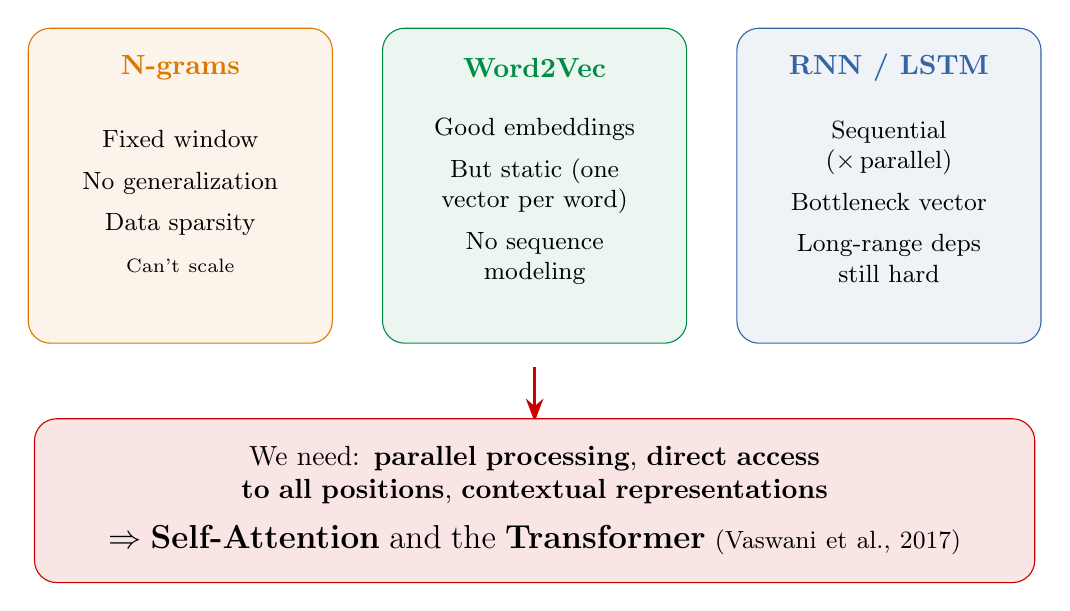
\begin{tikzpicture}
  % Three columns summarizing limitations
  \node[draw=orange1, fill=orange1!8, rounded corners=8pt, minimum height=4cm, text width=3.3cm, align=center, inner sep=8pt] at (-4.5, 1) {};
  \node[font=\normalsize\bfseries, text=orange1] at (-4.5, 2.5) {N-grams};
  \node[font=\small, text width=3cm, align=center] at (-4.5, 0.8) {
    Fixed window\\[4pt]
    No generalization\\[4pt]
    Data sparsity\\[4pt]
    {\scriptsize Can't scale}
  };

  \node[draw=paramgreen, fill=paramgreen!8, rounded corners=8pt, minimum height=4cm, text width=3.3cm, align=center, inner sep=8pt] at (0, 1) {};
  \node[font=\normalsize\bfseries, text=paramgreen] at (0, 2.5) {Word2Vec};
  \node[font=\small, text width=3cm, align=center] at (0, 0.8) {
    Good embeddings\\[4pt]
    But static (one\\vector per word)\\[4pt]
    No sequence\\modeling
  };

  \node[draw=popblue, fill=popblue!8, rounded corners=8pt, minimum height=4cm, text width=3.3cm, align=center, inner sep=8pt] at (4.5, 1) {};
  \node[font=\normalsize\bfseries, text=popblue] at (4.5, 2.5) {RNN / LSTM};
  \node[font=\small, text width=3cm, align=center] at (4.5, 0.8) {
    Sequential ($\times$\,parallel)\\[4pt]
    Bottleneck vector\\[4pt]
    Long-range deps\\still hard
  };

  % Arrow down
  \draw[-Stealth, very thick, sampred] (0, -1.3) -- (0, -2);

  % What we need
  \node[draw=sampred, fill=sampred!10, rounded corners=8pt, text width=12cm, align=center, inner sep=10pt, font=\normalsize] at (0, -3) {
    We need: \textbf{parallel processing}, \textbf{direct access to all positions}, \textbf{contextual representations}\\[6pt]
    {\large $\Rightarrow$ \textbf{Self-Attention} and the \textbf{Transformer}} {\small (Vaswani et al., 2017)}
  };
\end{tikzpicture}
\end{center}
\end{frame}

% ============================================================
% WORD2VEC TRAINING
% ============================================================
\begin{frame}
\frametitle{Word2Vec --- training tricks}
\vspace{-0.2cm}
\begin{center}
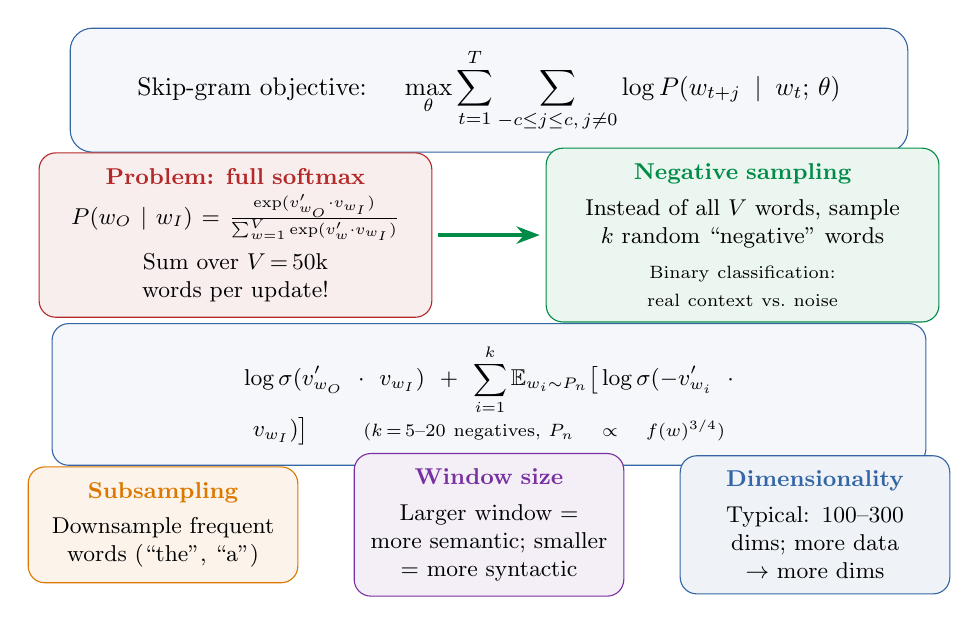
\begin{tikzpicture}[scale=0.92, transform shape]
  % Skip-gram objective
  \node[draw=popblue, fill=popblue!5, rounded corners=8pt, inner sep=8pt, text width=11cm, align=center] at (0, 3) {
    {\normalsize Skip-gram objective:} \quad $\displaystyle \max_\theta \sum_{t=1}^{T} \sum_{-c \le j \le c,\, j\neq 0} \log P(w_{t+j} \mid w_t;\, \theta)$
  };

  % Softmax problem
  \node[draw=warnred, fill=warnred!8, rounded corners=6pt, text width=5cm, align=center, inner sep=6pt, font=\small] at (-3.5, 1) {
    \textbf{\textcolor{warnred}{Problem: full softmax}}\\[3pt]
    $P(w_O \mid w_I) = \frac{\exp(v'_{w_O} \cdot v_{w_I})}{\sum_{w=1}^{V} \exp(v'_w \cdot v_{w_I})}$\\[4pt]
    Sum over $V$\,=\,50k words per update!
  };

  % Arrow
  \draw[-Stealth, very thick, paramgreen] (-0.7, 1) -- (0.7, 1);

  % Negative sampling
  \node[draw=paramgreen, fill=paramgreen!8, rounded corners=6pt, text width=5cm, align=center, inner sep=6pt, font=\small] at (3.5, 1) {
    \textbf{\textcolor{paramgreen}{Negative sampling}}\\[3pt]
    Instead of all $V$ words, sample $k$ random ``negative'' words\\[3pt]
    {\scriptsize Binary classification: real context vs.\ noise}
  };

  % NEG objective
  \node[draw=popblue, fill=popblue!5, rounded corners=6pt, inner sep=8pt, text width=11.5cm, align=center, font=\small] at (0, -1.2) {
    $\displaystyle \log \sigma(v'_{w_O} \cdot v_{w_I}) + \sum_{i=1}^{k} \mathbb{E}_{w_i \sim P_n} \big[\log \sigma(-v'_{w_i} \cdot v_{w_I})\big]$
    \qquad {\scriptsize ($k$\,=\,5--20 negatives, $P_n \propto f(w)^{3/4}$)}
  };

  % Other tricks
  \node[draw=orange1, fill=orange1!8, rounded corners=6pt, text width=3.3cm, align=center, inner sep=6pt, font=\small] at (-4.5, -3) {
    \textbf{\textcolor{orange1}{Subsampling}}\\[3pt]
    Downsample frequent words (``the'', ``a'')
  };
  \node[draw=violet1, fill=violet1!8, rounded corners=6pt, text width=3.3cm, align=center, inner sep=6pt, font=\small] at (0, -3) {
    \textbf{\textcolor{violet1}{Window size}}\\[3pt]
    Larger window = more semantic; smaller = more syntactic
  };
  \node[draw=popblue, fill=popblue!8, rounded corners=6pt, text width=3.3cm, align=center, inner sep=6pt, font=\small] at (4.5, -3) {
    \textbf{\textcolor{popblue}{Dimensionality}}\\[3pt]
    Typical: 100--300 dims; more data $\rightarrow$ more dims
  };
\end{tikzpicture}
\end{center}
\end{frame}

% ============================================================
% GLOVE & FASTTEXT
% ============================================================
\begin{frame}
\frametitle{Beyond Word2Vec --- GloVe \& FastText}
\vspace{-0.4cm}
\begin{center}
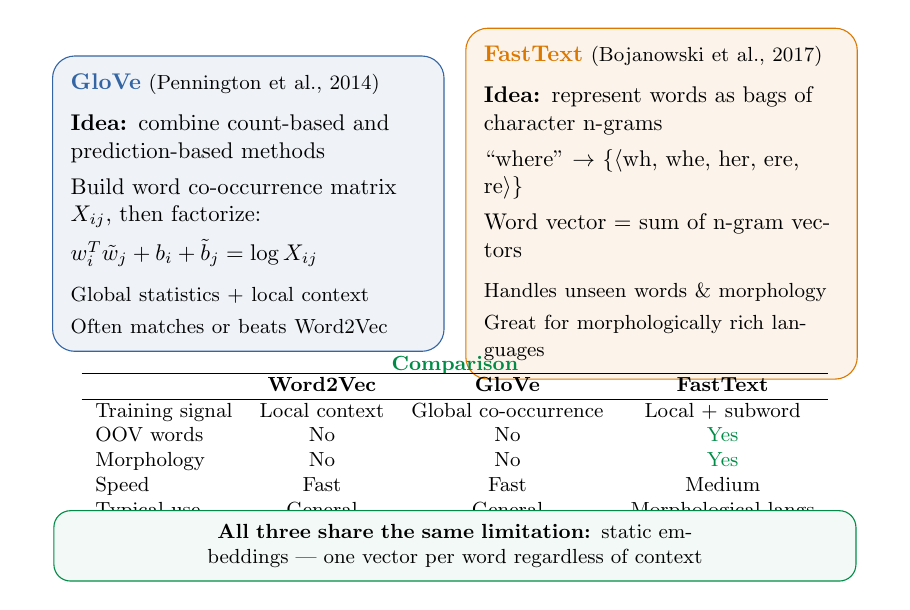
\begin{tikzpicture}[scale=0.82, transform shape]
  % GloVe section
  \node[draw=popblue, fill=popblue!8, rounded corners=8pt, text width=5.5cm, align=left, inner sep=8pt] at (-3.2, 2) {
    \textbf{\textcolor{popblue}{\normalsize GloVe}} {\small (Pennington et al., 2014)}\\[6pt]
    \textbf{Idea:} combine count-based and prediction-based methods\\[4pt]
    Build word co-occurrence matrix $X_{ij}$, then factorize:\\[4pt]
    $w_i^T \tilde{w}_j + b_i + \tilde{b}_j = \log X_{ij}$\\[6pt]
    {\small Global statistics + local context}\\[2pt]
    {\small Often matches or beats Word2Vec}
  };

  % FastText section
  \node[draw=orange1, fill=orange1!8, rounded corners=8pt, text width=5.5cm, align=left, inner sep=8pt] at (3.2, 2) {
    \textbf{\textcolor{orange1}{\normalsize FastText}} {\small (Bojanowski et al., 2017)}\\[6pt]
    \textbf{Idea:} represent words as bags of character n-grams\\[4pt]
    ``where'' $\rightarrow$ \{$\langle$wh, whe, her, ere, re$\rangle$\}\\[4pt]
    Word vector = sum of n-gram vectors\\[6pt]
    {\small Handles unseen words \& morphology}\\[2pt]
    {\small Great for morphologically rich languages}
  };

  % Comparison
  \node[font=\small\bfseries, text=paramgreen] at (0, -0.5) {Comparison};

  % Table
  \node[font=\small, text width=13cm, align=center] at (0, -1.8) {
    \begin{tabular}{l c c c}
    \hline
    & \textbf{Word2Vec} & \textbf{GloVe} & \textbf{FastText} \\
    \hline
    Training signal & Local context & Global co-occurrence & Local + subword \\
    OOV words & No & No & \textcolor{paramgreen}{Yes} \\
    Morphology & No & No & \textcolor{paramgreen}{Yes} \\
    Speed & Fast & Fast & Medium \\
    Typical use & General & General & Morphological langs \\
    \hline
    \end{tabular}
  };

  % Bottom note
  \node[draw=paramgreen, fill=paramgreen!5, rounded corners=6pt, text width=12cm, align=center, inner sep=6pt, font=\small] at (0, -3.3) {
    \textbf{All three share the same limitation:} static embeddings --- one vector per word regardless of context
  };
\end{tikzpicture}
\end{center}
\end{frame}

% ============================================================
% FURTHER READING
% ============================================================
\begin{frame}
\frametitle{Further reading}
\vspace{-0.4cm}
\begin{center}
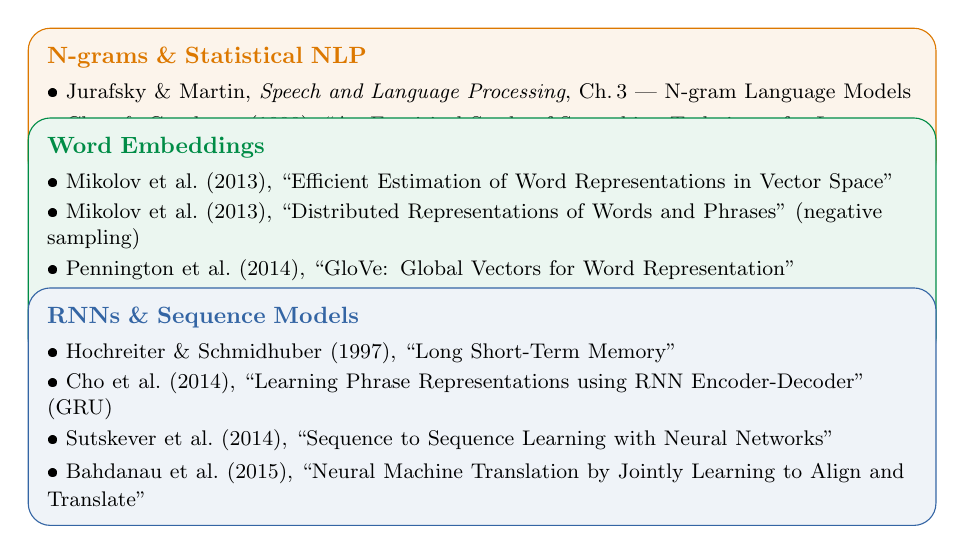
\begin{tikzpicture}[scale=0.85, transform shape]
  % N-grams & Statistical NLP
  \node[draw=orange1, fill=orange1!8, rounded corners=8pt, text width=13cm, align=left, inner sep=8pt] at (0, 2.5) {
    \textbf{\textcolor{orange1}{N-grams \& Statistical NLP}}\\[4pt]
    {\small
    \textbullet~Jurafsky \& Martin, \emph{Speech and Language Processing}, Ch.\,3 --- N-gram Language Models\\[2pt]
    \textbullet~Chen \& Goodman (1999), ``An Empirical Study of Smoothing Techniques for Language Modeling''
    }
  };

  % Word Embeddings
  \node[draw=paramgreen, fill=paramgreen!8, rounded corners=8pt, text width=13cm, align=left, inner sep=8pt] at (0, 0.5) {
    \textbf{\textcolor{paramgreen}{Word Embeddings}}\\[4pt]
    {\small
    \textbullet~Mikolov et al.\ (2013), ``Efficient Estimation of Word Representations in Vector Space''\\[2pt]
    \textbullet~Mikolov et al.\ (2013), ``Distributed Representations of Words and Phrases'' (negative sampling)\\[2pt]
    \textbullet~Pennington et al.\ (2014), ``GloVe: Global Vectors for Word Representation''\\[2pt]
    \textbullet~Bojanowski et al.\ (2017), ``Enriching Word Vectors with Subword Information'' (FastText)
    }
  };

  % RNNs & Sequence Models
  \node[draw=popblue, fill=popblue!8, rounded corners=8pt, text width=13cm, align=left, inner sep=8pt] at (0, -2) {
    \textbf{\textcolor{popblue}{RNNs \& Sequence Models}}\\[4pt]
    {\small
    \textbullet~Hochreiter \& Schmidhuber (1997), ``Long Short-Term Memory''\\[2pt]
    \textbullet~Cho et al.\ (2014), ``Learning Phrase Representations using RNN Encoder-Decoder'' (GRU)\\[2pt]
    \textbullet~Sutskever et al.\ (2014), ``Sequence to Sequence Learning with Neural Networks''\\[2pt]
    \textbullet~Bahdanau et al.\ (2015), ``Neural Machine Translation by Jointly Learning to Align and Translate''
    }
  };
\end{tikzpicture}
\end{center}
\end{frame}

% ============================================================
% QUESTIONS
% ============================================================
\begin{frame}
\begin{center}
\vspace{2cm}
{\Huge \textcolor{popblue}{Questions?}}

\vspace{1cm}
{\large Next: The Transformer Architecture}
\end{center}
\end{frame}

\end{document}
